\documentclass{article}
\usepackage{graphicx}
\usepackage{blochsphere}
\usepackage{tikz}
\usetikzlibrary{calc}
\usepackage{amsmath}
\usepackage{amssymb}
\usepackage{amsfonts}
\usepackage{tikz}
\usetikzlibrary{positioning,arrows,calc,math,angles,quotes}
\usepackage{blochsphere}
\usepackage{braket}
\usepackage[x11names]{xcolor}
\usepackage[paperwidth=16in, paperheight=9in, margin=0cm]{geometry} % 16:9 aspect ratio, no margins
\usepackage{textpos} % For absolute positioning of content

% Define background and text color
\definecolor{mycolor}{RGB}{27, 27, 27}
\pagecolor{mycolor}
\color{white}

\begin{document}
\pagenumbering{gobble}

% Start positioning the Bloch sphere wherever you like on the page
\begin{textblock*}{\textwidth}(0cm,0.5cm) % Adjust position (x, y) here
    \centering
    %%%% Change these parameters to change the position of psi, or the size/rotation of the sphere
\def\rotationSphere{-110}
\def\radiusSphere{5cm}
\def\psiLat{45}
\def\psiLon{45}
\def\textSize{\large} % Control text size here

\begin{blochsphere}[radius=\radiusSphere, opacity=0.025, rotation=\rotationSphere]
  \drawBallGrid[style={opacity=.3}]{30}{45}
  % Draw the sphere...
  \drawLongitudeCircle[]{\rotationSphere}
  \drawLatitudeCircle[style={dashed}]{0}
  
  % Define the different points on the Bloch sphere
  \labelLatLon{ket0}{90}{0};
  \labelLatLon{ket1}{-90}{0};
  \labelLatLon{ket2}{45}{0};
  \labelLatLon{ketminus}{0}{180};
  \labelLatLon{ketplus}{0}{0};
  \labelLatLon{ketpluspi2}{0}{-90};
  \labelLatLon{ketplus3pi2}{0}{-270};
  \labelLatLon{psi}{\psiLat}{-\psiLon};
  
  % Draw and label the axes
  
  \draw[-latex] (0,0) -- (ket0) node[above, inner sep=.5mm] at (ket0) {\textSize $z \, \ket{1}$};
  
  \draw[-latex] node[below, inner sep=1.5mm] at (ket1) {\textSize $-z \, \ket{0}$};
  
  \draw[-latex] (0,0) -- (ketplus) node[below left,inner sep=.5mm] at (ketplus) {\textSize $x \, \ket{+}$};
  
  \draw[-latex] node[above right,inner sep=.5mm] at (ketminus) {\textSize $-x \, \ket{-}$};
  
  \draw[-latex] (0,0) -- (ketpluspi2) node[right,inner sep=3mm] at (ketpluspi2) {\textSize $y \, \ket{+i}$};
  
  \draw[-latex] node[left,inner sep=2.5mm] at (ketplus3pi2) {\textSize $-y \, \ket{-i}$};
  
  % Draw |psi>
  \draw[-latex] (0,0) -- (psi) node[above]{\textSize $\ket{\psi}$};

  % Draw the angles
  \coordinate (origin) at (0,0);
  {
    \setDrawingPlane{0}{0}
    \draw[current plane, dashed] (0,0) -- (-90+\psiLon:{cos(\psiLat)*\radiusSphere}) coordinate (psiProjectedEquat) -- (psi);
    \pic[current plane, draw, fill=orange!50, fill opacity=.5, text opacity=1, "\textSize $\phi$", angle eccentricity=2.2]{angle=ketplus--origin--psiProjectedEquat};
  }
  { \setLongitudinalDrawingPlane{\psiLon}
    \pic[current plane, draw, fill=orange!50, fill opacity=.5, text opacity=1, "\textSize $\theta$", angle eccentricity=1.5]{angle=psi--origin--ket0};
  }
\end{blochsphere}

\end{textblock*}


\begin{textblock*}{\textwidth}(0cm,13cm) % Adjust position (x, y) here
    \centering
    \Large $i \hbar \frac{\partial}{\partial t} \ket{\psi (t)} = \hat{H} \ket{\psi (t)}$
    \vspace{10pt}


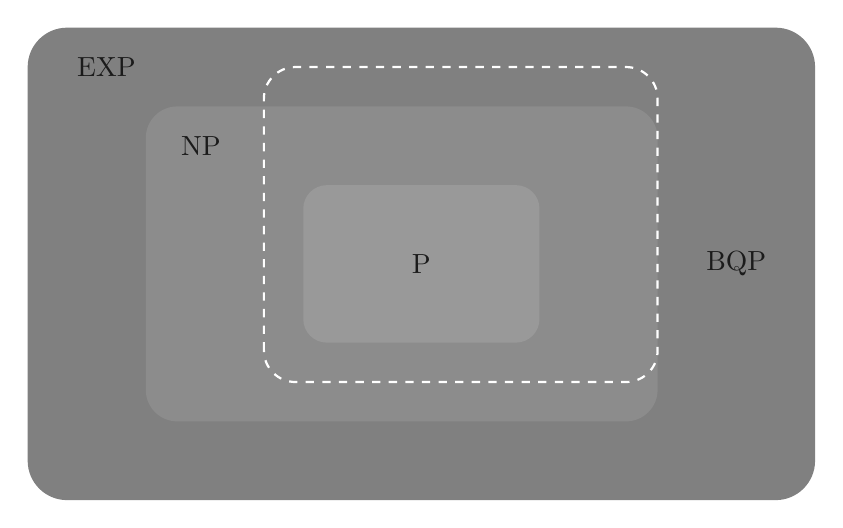
\begin{tikzpicture}
    % EXP Problems container (outermost rounded rectangle)
    \fill[gray!100, rounded corners=0.5cm] (-5, -2.5) rectangle (5, 3.5);
    \node[mycolor] at (-4, 3) {EXP};

    % NP Problems container (rounded rectangle inside EXP)
    \fill[gray!90, rounded corners=0.4cm] (-3.5, -1.5) rectangle (3, 2.5);
    \node[mycolor] at (-2.8, 2) {NP};

    % P Problems container (smallest rounded rectangle inside NP)
    \fill[gray!80, rounded corners=0.3cm] (-1.5, -0.5) rectangle (1.5, 1.5);
    \node[mycolor] at (0, 0.5) {P};

    % BQP boundary (dashed, closed rounded rectangle overlapping NP and enclosing P)
    \draw[dashed, rounded corners=0.4cm, thick, white] (-2, -1) rectangle (3, 3);
    \node[mycolor] at (4, .5) {BQP};

\end{tikzpicture}
    
\end{textblock*}




\end{document}
